Thomson问题指的是求球面上$N$个电子的势能极小值以及相应位型。
通过取$\frac{e^2}{4\pi\epsilon_0} = 1$,式子可以得到简化。
本题要求对$N = 2, 3, \cdots, 64$的情况进行求解。
此外,还需要对$N = 12$的情况分析稳定构型、计算小振动简正频率。

使用球坐标,球坐标下两点$(\theta_1, \phi_1)$与$(\theta_2, \phi_2)$的欧式直线距离为
\begin{multline}
    r_{12} = 2\sqrt{\sin^2{\frac{\theta_1 - \theta_2}{2}} + \sin{\theta_1}\sin{\theta_2}\sin^2{\frac{\phi_1 - \phi_2}{2}}}\\
    = \sqrt{2\qty(1-\cos(\theta_1 - \theta_2) + \sin{\theta_1}\sin{\theta_2}(1-\cos(\phi_1 - \phi_2)))}.
\end{multline}
那么,系统的总势能
\begin{equation}
    V = \frac{1}{2}\sum_{i\neq j}\frac{1}{r_{ij}} = \sum_{i < j}\frac{1}{r_{ij}}.
\end{equation}
我们需要求解其最小值。

求解的程序源代码为\texttt{4\_Thomson.cpp}。
注意到,系统实际上有三个多余自由度(即决定系统朝向的三个欧拉角)。
我选择将其中一个电子固定在$\qty(\frac{\pi}{2}, 0)$处,以减小优化问题的维数。
位型使用数组表示,依次按顺序存放各个电子的$\theta$与$\phi$。

\section{求解最小势能\texorpdfstring{$V_\text{min}(N)$}{Vmin(N)}}
使用Polak-Ribiere的非线性共轭梯度法求解最小势能,初始电子位型为球面上随机均匀分布。
由于可能的初值敏感,对每个$N$使用不同的随机初值计算5遍取最小值。
求解的函数\texttt{solve<N>()}如下,其接受随机数引擎\texttt{ran},详细输出的输出流\texttt{os}以及重复次数\texttt{n}。
{
    \linespread{1.0}
    \lstinputlisting[linerange=beg:solve-end:solve]{4_Thomson.cpp}
}
其将向\texttt{os}输出当前电子数\texttt{N}以及\texttt{n}次计算的结果,并最后附上最小的势能。
同时,其也将当前电子数\texttt{N}以及最小势能向\texttt{cerr}输出。

\texttt{solve<N>()}首先定义初始位型\texttt{x0}。
使用随机数发生器,使各个初始的$\theta$的$\cos{\theta}$在$[-1, 1)$上随机均匀分布,各个初始的$\phi$在$[0, 2\pi)$上随机均匀分布。

随后使用\texttt{conj\_grad<>()}函数求最小值。
该函数接受待优化的势函数\texttt{potential<>()}、势函数的梯度\texttt{grad\_potential<>()}、初始值\texttt{x0}、以及每次迭代后要对\texttt{x0}做的修改\texttt{modify<>()}。
\texttt{modify<>()}将所有$\theta$和$\phi$对$2\pi$取余,以将\texttt{x0}限制在离原点最近的周期内,以避免x0漂至过远的地方影响精度。
其他函数会在后面逐一介绍。
\texttt{modify<>()}见下:
{
    \linespread{1.0}
    \lstinputlisting[linerange=beg:modify-end:modify]{4_Thomson.cpp}
}
得到解\texttt{res}后,计算该点处的势能存入\texttt{solutions}并输出至\texttt{os}。
在函数的最后,找到\texttt{solutions}中最小的解并输出。

\subsection{共轭梯度法}
\texttt{conj\_grad<>()}基于Polak-Ribiere算法,位于\texttt{misc/optimize.h}中,如下
{
    \linespread{1.0}
    \lstinputlisting[linerange=beg:cg-end:cg]{../misc/optimize.h}
}
其中,线性搜索步长$\alpha$使用Kiefer黄金分割搜索。
使用$\lambda$表达式将势函数包装为搜索方向上的一维函数,然后传给一维优化函数\texttt{minimize1d\_kiefer()}搜索。
最开始的搜索上限为$1/g$,其中$g$为初始梯度的模。
此后,搜索上限为上一轮得到的$\alpha$的$\phi = \frac{\sqrt{5}+1}{2} \approx 1.618$倍。
另外,若单次的搜索结果过于接近上界,会扩大上界,重新搜索。

搜索方向$\vb{d}$的迭代方法为
\begin{gather}
    \vb{d}_{i+1} = -\vb{g}_{i+1} + \beta_{i+1}\vb{d}_{i},\\
    \beta_{i+1} = \frac{\vb{g}^T_{i+1}(\vb{g}_{i+1}-\vb{g}_{i})}{\vb{g}^T_{i}\vb{g}_{i}}.
\end{gather}
其中$\vb{g}_{i+1}$为当前梯度。

判停标准为\texttt{x0}的增量的模与\texttt{x0}的模之比足够小。
\subsection{势函数}
函数\texttt{potential<>()}见下
{
    \linespread{1.0}
    \lstinputlisting[linerange=beg:potential-end:potential]{4_Thomson.cpp}
}
即将各对的
\begin{equation}
\frac{1}{r_{ij}} = \frac{1}{\sqrt{2(1-\cos(\theta_i - \theta_j) + \sin{\theta_i}\sin{\theta_j}(1-\cos(\phi_i - \phi_j)))}}
\end{equation}
算出并求和。
此外,在一开始对固定点$\qty(\frac{\pi}{2}, 0)$的贡献进行了计算。

为减少重复调用函数的开销,定义了一些临时变量。
\subsection{势函数的梯度}\label{ssec:grad}
注意到,$\frac{1}{r_{ij}}$只对第$i$与第$j$个电子的这四个参数方向上的梯度有贡献。
有
\begin{align}
    \pdv{\theta_i}\frac{1}{r_{ij}} &{}= -\frac{1}{r^3_{ij}}(\sin(\theta_i - \theta_j) + \cos{\theta_i}\sin{\theta_j}(1-\cos(\phi_i - \phi_j))),\\
    \pdv{\phi_i}\frac{1}{r_{ij}} &{}= -\frac{1}{r^3_{ij}}\sin{\theta_i}\sin{\theta_j}\sin(\phi_i - \phi_j),\\
    \pdv{\theta_j}\frac{1}{r_{ij}} &{}= -\frac{1}{r^3_{ij}}(-\sin(\theta_i - \theta_j) + \sin{\theta_i}\cos{\theta_j}(1-\cos(\phi_i - \phi_j))),\\
    \pdv{\phi_j}\frac{1}{r_{ij}} &{}= -\pdv{\phi_i}\frac{1}{r_{ij}}.
\end{align}

那么,只需要仍然对各对$r_{ij}$遍历,将它们的贡献加到结果相应的四个方向上即可。
\texttt{grad\_potential<>()}的实现如下
{
    \linespread{1.0}
    \lstinputlisting[linerange=beg:grad_potential-end:grad_potential]{4_Thomson.cpp}
}
为减少重复调用函数的开销,定义了一些临时变量。

\subsection{计算结果}
共轭梯度法整体性能较好。
在$N=64$时,一般可在300至400轮迭代后得到结果,用时5 s左右。
$N=2, 3, \cdots, 64$的计算结果见\autoref{tab:potential_min};
原始数据见\texttt{4\_Thomson\_1\_complete}。

\begin{table}
\centering
\caption{最小势能计算结果}
\label{tab:potential_min}
\begin{tabular}{cr@{.}l|cr@{.}l}
\toprule
$N$ & \multicolumn{2}{c|}{$V_\text{min}$} & $N$ & \multicolumn{2}{c}{$V_\text{min}$} \\ \midrule
2 & 0&5000000000000000 & 34 & 468&9048532813456 \\
3 & 1&732050807568877 & 35 & 498&5698724906555 \\
4 & 3&674234614174767 & 36 & 529&1224083761713 \\
5 & 6&474691494688162 & 37 & 560&6188877311088 \\
6 & 9&985281374238570 & 38 & 593&0385035664638 \\
7 & 14&45297741422138 & 39 & 626&3890090168419 \\
8 & 19&67528786123277 & 40 & 660&6752788346374 \\
9 & 25&75998653126986 & 41 & 695&9167443418991 \\
10 & 32&71694946014762 & 42 & 732&0781075437027 \\
11 & 40&59645050819067 & 43 & 769&1908464593217 \\
12 & 49&16525305762881 & 44 & 807&1742630850263 \\
13 & 58&85323061170261 & 45 & 846&1884010611892 \\
14 & 69&30636329662660 & 46 & 886&1671136392418 \\
15 & 80&67024411429404 & 47 & 927&0592706797588 \\
16 & 92&91165530254507 & 48 & 968&7134553437978 \\
17 & 106&0504048286190 & 49 & 1011&557182653595 \\
18 & 120&0844674474926 & 50 & 1055&182314726304 \\
19 & 135&0894675566883 & 51 & 1099&819290318931 \\
20 & 150&8815683337568 & 52 & 1145&418964319396 \\
21 & 167&6416223992741 & 53 & 1191&922290417235 \\
22 & 185&2875361493095 & 54 & 1239&361474729189 \\
23 & 203&9301906628806 & 55 & 1287&772720782750 \\
24 & 223&3470740518091 & 56 & 1337&094945275748 \\
25 & 243&8127602987741 & 57 & 1387&383229253046 \\
26 & 265&1333263173655 & 58 & 1438&618250640455 \\
27 & 287&3026150330439 & 59 & 1490&773335278781 \\
28 & 310&4915423582055 & 60 & 1543&830400976449 \\
29 & 334&6344399204337 & 61 & 1597&941830199204 \\
30 & 359&6039459037797 & 62 & 1652&909409898416 \\
31 & 385&5308380633008 & 63 & 1708&879681503394 \\
32 & 412&2612746505320 & 64 & 1765&802577927376 \\
33 & 440&2040574476876 &  & \multicolumn{2}{c}{}\\ \bottomrule
\end{tabular}
\end{table}

计算中发现,$N\in\{47,53,56,58\}$时得到的结果与Wikipedia上的结果\footnote{\url{https://en.wikipedia.org/w/index.php?title=Thomson_problem&oldid=951524019}}相差较大,于是重新对其进行计算。
重新计算的结果已填入\autoref{tab:potential_min}中,原始数据见\texttt{4\_Thomson\_1\_append}。

\section{\texorpdfstring{$N=12$}{N = 12}时的小振动}
本节的代码示例输出见\texttt{4\_Thomson\_2}。

重新求解$N=12$时的位型,代码如下
{
    \linespread{1.0}
    \lstinputlisting[linerange=beg:12calc-end:12calc]{4_Thomson.cpp}
}
将输出求得的最小势能以供检查。
求得的最小势能为$49.165\,253\,057\,628\,87$,正确。

\subsection{检查电子构型是否为正二十面体}
正二十面体(\autoref{fig:icosahedron})有30条等长的棱。
在棱长为$a$时,其外接球的半径为\footnote{\url{https://en.wikipedia.org/w/index.php?title=Regular_icosahedron&oldid=942166818}}
\begin{equation}
    r = \frac{a}{4} \sqrt{10+2\sqrt{5}} \approx 0.951\,056\,5163\,a.
\end{equation}

\begin{figure}
    \centering
    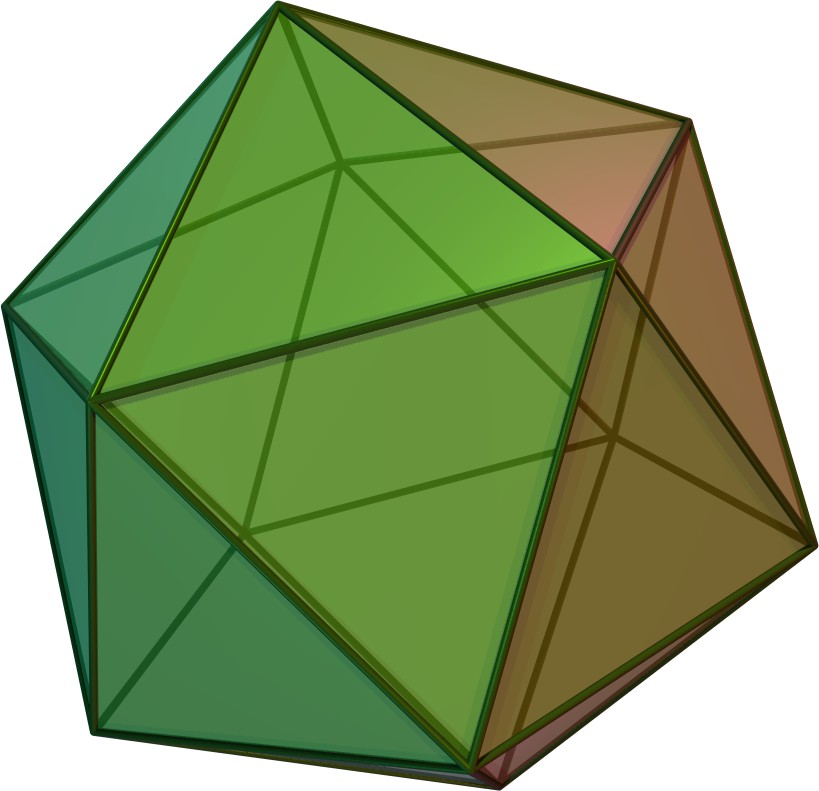
\includegraphics[width=.5\textwidth]{Icosahedron.jpg}
    \caption{正二十面体(\textit{Wikimedia Commons},按照CC BY-SA 3.0发布。\url{https://commons.wikimedia.org/w/index.php?title=File:Icosahedron.jpg&oldid=222275944})}
    \label{fig:icosahedron}
\end{figure}

为判断是否得到了正二十面体,我们可以将解得的res中各对电子之间的距离中最小的30个进行对比,如果它们都很接近$\frac{4}{\sqrt{10+2\sqrt{5}}} \approx 1.051\,462\,2242$,那么可以认为我们得到了一个正二十面体。

函数\texttt{distances<>()}会返回各对电子的间距组成的\texttt{vector}。
其基本基于\texttt{potential<>()}的代码,定义如下
{
    \linespread{1.0}
    \lstinputlisting[linerange=beg:distances-end:distances]{4_Thomson.cpp}
}
只是将\texttt{potential<>()}中的增加势能改为推入距离,并在最后排序。

随后,输出最小距离以及第30小的距离:
{
    \linespread{1.0}
    \lstinputlisting[linerange=end:12calc-end:icosahedron]{4_Thomson.cpp}
}
得到的结果分别是$1.051\,462\,071\,022\,363$与$1.051\,462\,360\,844\,809$。
两者都与$\frac{4}{\sqrt{10+2\sqrt{5}}} \approx 1.051\,462\,2242$十分接近,说明确实得到了一个正二十面体。

\subsection{求解小振动}
函数$f(\vb{x})$在极小值点$\vb{x}^*$附近(记$\vb{x} = \vb{x}^* + \vb{q}$)可展开为
\begin{equation}
    f(\vb{x}) = f(\vb{x}^*) + \frac{1}{2}\vb{q}^T\vb{H}(\vb{x}^*)\vb{q},
\end{equation}
其中黑塞矩阵
\begin{equation}
    \vb{H}(\vb{x}^*) = \qty{H_{ij}} = \qty{\pdv{f}{x_i}{x_j}}.
\end{equation}
显然,$\vb{H}(\vb{x}^*)$对称且在极小值处正定。
本问题中,由于三个额外自由度的存在,$\vb{H}(\vb{x}^*)$半正定,有三个特征值为0。

因此,在势能极小点附近,可展开为(使用爱因斯坦求和规则)
\begin{equation}
    V = \frac{1}{2}q_iV_{ij}q_j + V_0.
\end{equation}
加上动能展开式,能量守恒可写为
\begin{equation}
    \frac{1}{2}q_iV_{ij}q_j
    + \frac{1}{2}\dot{q}_iT_{ij}\dot{q}_j
    = C.
\end{equation}

两边对时间求导,考虑到$\qty{V_{ij}}$与$\qty{T_{ij}}$对称,可有
\begin{equation}
    \dot{q}_i
    \qty(V_{ij}q_j + T_{ij}\ddot{q}_j)
    = 0.
\end{equation}
又因为$\dot{q}$任意,可得
\begin{equation}
    V_{ij}q_j + T_{ij}\ddot{q}_j = 0.
\end{equation}
对于以$\omega$振动的本征简谐解,有
\begin{equation}
    V_{ij}q_j = \omega^2T_{ij}q_j,\quad
    \vb{V}\vb{q} = \omega^2 \vb{T}\vb{q},
\end{equation}
为一个广义本征值问题。

由于$\vb{V}, \vb{T}$都是半正定的,必均可对角化。我们假设$\vb{T}$可被正交矩阵$\vb{G}$对角化,有
\begin{equation}
    \vb{T} = \vb{G}^T\vb{T}\vb{G},
\end{equation}
那么
\begin{equation}
    \vb{G}\vb{V}\vb{G}^T\cdot\vb{G}\vb{q} = \omega^2\vb{D}_T\vb{G}\vb{T}.
\end{equation}

由于$\vb{T}$半正定,$\vb{D}_T$所有元素非负,可写为
\begin{equation}
    \vb{D}_T = \sqrt{\vb{D}_T}\sqrt{\vb{D}_T},
\end{equation}
有
\begin{equation}
    \sqrt{\vb{D}_T}^{-1}\vb{G}\vb{V}\vb{G}^T\sqrt{\vb{D}_T}^{-1}
    \cdot \sqrt{\vb{D}_T}\vb{G}\vb{q}
    = \omega^2\sqrt{\vb{D}_T}\vb{G}\vb{q}.
\end{equation}
问题变成了求
\begin{equation}
    \vb{V}' = \sqrt{\vb{D}_T}^{-1}\vb{G}\vb{V}\vb{G}^T\sqrt{\vb{D}_T}
\end{equation}
的所有特征值$\omega^2_i$。

本题中,
\begin{equation}
    T = \sum_{i}\frac{1}{2}(\dot{\theta}^2 + \dot{\phi}^2\sin^2{\theta}),
\end{equation}
$\vb{T}$已经是正定的,故只需求出黑塞矩阵$\vb{V}$,然后求$\vb{V}' = \sqrt{\vb{T}}^{-1}\vb{V}\sqrt{\vb{T}}$的本征值。

\subsubsection{黑塞矩阵}
前面在\autoref{ssec:grad} 已经求出了势能的梯度。
注意到,对梯度我们相当于得到了
\begin{equation}
    \pdv{q_i}\frac{1}{r} = \frac{A_i}{r^3}.
\end{equation}
那么黑塞矩阵便可拆成两部分
\begin{equation}\label{eq:hessian}
    \pdv{}{q_i}{q_j} \frac{1}{r}
    = \frac{3A_iA_j}{r^5} + \frac{1}{r^3}\pdv{A_i}{q_j}.
\end{equation}

黑塞矩阵的第一部分是现成的,下面着重说一下第二部分。
对于向量$\qty[\theta_i, \phi_i, \theta_j, \phi_j]$,黑塞矩阵的第二部分可写为(矩阵对称,仅列出上半部分)
\begin{equation}
    \frac{1}{r^3_{ij}}\mqty[
        \alpha& \beta&  \gamma& -\beta\\
        &   \delta& \epsilon&   -\delta\\
        &&  \alpha& -\epsilon\\
        &&& \delta
    ],
\end{equation}
其中
\begin{align}
    \alpha &{}= -\cos(\theta_i - \theta_j) + \sin{\theta_i}\sin{\theta_j}(1-\cos(\phi_i - \phi_j)),\\
    \beta &{}= -\cos{\theta_i}\sin{\theta_j}\sin(\phi_i - \phi_j),\\
    \gamma &{}= \cos(\theta_i - \theta_j) - \cos{\theta_i}\cos{\theta_j}(1-\cos(\phi_i - \phi_j)),\\
    \delta &{}= -\sin{\theta_i}\sin{\theta_j}\cos(\phi_i - \phi_j),\\
    \epsilon &{}= -\sin{\theta_i}\cos{\theta_j}\sin(\phi_i - \phi_j).
\end{align}

黑塞矩阵的计算函数如下
{
    \linespread{1.0}
    \lstinputlisting[linerange=beg:hessian_potential-end:hessian_potential]{4_Thomson.cpp}
}
其中大写字母开头的\texttt{Theta1}等变量即为 \eqref{eq:hessian} 中的$A_i$等。

由于之前计算极小值的时候固定了一个电子,在计算黑塞矩阵前要恢复这一自由度。
同时顺便将电子位型输出。
相应代码如下,完整的电子位型存储在\texttt{complete\_res}中。
{
    \linespread{1.0}
    \lstinputlisting[linerange=end:icosahedron-end:calc_hessian]{4_Thomson.cpp}
}

\subsubsection{本征值计算}
本人实现了双位移隐式QR算法,并用其计算本征值。
算法具体实现参见\texttt{misc/eigvals.h},下面仅简要说明一下思路。
首先介绍隐式QR定理\footnote{\url{http://math.ecnu.edu.cn/~jypan/Teaching/MatrixComp/slides_ch04_eig_nonsymm.pdf}}。

\begin{mythm}[隐式QR定理]
    设 $\vb{H} = \vb{Q}^T\vb{A}\vb{Q} \in \mathbb{R}^{n\times n} $是一个不可约上Hessenberg矩阵,其中$\vb{Q}\in \mathbb{R}^{n\times n}$是正交矩阵,则$\vb{Q}$的第 $2$ 至第$n$列均由$\vb{Q}$的第一列所唯一确定(可相差一个符号)
\end{mythm}

这样的话,就可以在实现QR算法的时候,只算出$\vb{Q}$的第一列,然后直接将原矩阵更改为下一个迭代,而不需要显式地进行QR分解,从而更为高效。

因此,本征值计算函数\texttt{eig\_vals()}的内部便是:
\begin{compactenum}
    \item 使用函数\texttt{hessenberg()}将矩阵变为海森堡矩阵;
    \item 使用隐式QR算法\texttt{\_eig\_hessenberg()}将海森堡矩阵变为块对角矩阵;
    \item 处理块对角矩阵的块对角元,给出所有实本征值以及复本征值对的实部与虚部。
\end{compactenum}
\texttt{eig\_vals()}返回一个存储本征值的\texttt{array}与标记复本征值位置的\texttt{vector}。
若本征值都是实的,则\texttt{vector}为空。

\subsubsection{计算结果}
由前面讨论,动能矩阵$\vb{T}$已经是对角的。
通过计算其平方根的逆,然后作用在$\vb{V}$的两侧,可以得到我们最终要求本征值的矩阵$\vb{V}'$。
{
    \linespread{1.0}
    \lstinputlisting[linerange=end:calc_hessian-end:calc_V_prime]{4_Thomson.cpp}
}
现在,\texttt{hessian}为$\vb{V}'$。

计算本征值,判断是否有复本征值。
如果没有,将本征值排序并输出。
{
    \linespread{1.0}
    \lstinputlisting[linerange=end:calc_V_prime-end:eigs]{4_Thomson.cpp}
}

运行结果表明,不存在复的本征值,所有本征值见\autoref{tab:omegas}。
表中也列出了小振动的角频率与简并度。
最小的角频率十分接近0,对应的是平动自由度,简并度为3。

\begin{table}
\centering
\caption{$N=12$时系统在极小值附近振动的角频率}
\label{tab:omegas}
\begin{tabular}{llc}
\toprule
\multicolumn{1}{c}{$\omega^2$} & \multicolumn{1}{c}{$\omega = \sqrt{\overline{\omega^2}}$} & 简并度 \\ \midrule
\multicolumn{1}{@{$-$}l}{6.266861164308746e$-$08} & \multirow{3}{*}{2.0735364285199273e$-$05} & \multirow{3}{*}{3} \\
1.332267629550188e$-$15 &  &  \\
6.395847630693958e$-$08 &  &  \\\midrule
0.9071635997689073 & \multirow{5}{*}{0.95245151613015140} & \multirow{5}{*}{5} \\
0.9071636643108395 &  &  \\
0.9071637783464412 &  &  \\
0.9071641902009776 &  &  \\
0.9071642202659546 &  &  \\\midrule
2.150595912152278 & \multirow{4}{*}{1.4664913062020637} & \multirow{4}{*}{4} \\
2.150596305870100 &  &  \\
2.150597197066894 &  &  \\
2.150597589575669 &  &  \\\midrule
5.160417841630242 & \multirow{3}{*}{2.2716553286841448} & \multirow{3}{*}{3} \\
5.160417964471208 &  &  \\
5.160417990915761 &  &  \\\midrule
6.605910534349911 & \multirow{4}{*}{2.5701967499033627} & \multirow{4}{*}{4} \\
6.605910921739608 &  &  \\
6.605911773209189 &  &  \\
6.605912103556530 &  &  \\\midrule
6.967665806026027 & \multirow{5}{*}{2.6396337464435122} & \multirow{5}{*}{5} \\
6.967665881324974 &  &  \\
6.967666491315732 &  &  \\
6.967666659903127 &  &  \\
6.967666738247202 &  &  \\ \bottomrule
\end{tabular}
\end{table}
